\chapter{Method}

\section{Data}

The data is collected by Steady Health during a 4,5 month pilot study including 20 patients.
All patients are at least 18 years old and have been injecting insulin at least 1 year prior to the study.

Each patient are equipped with a CGM sensor for the entirety of the study.
For each patient, the CGM collected BG data at intervals of 1-5 minutes.
Patients will also log other events such as meals and exercise making those values accessible at some of the times steps.

\medskip
\begin{table}[ht!]
\begin{center}
  \begin{tabular}{lll}
  \textbf{Notation} &
  \textbf{Field} &
  \textbf{Format} \\
  \hline
  $P$ &
  Patient &
  Integer \\
  $t$ &
  Time &
  Date \\
  $t_{BG}$ &
  Glucose value at $t$ &
  Float \\
  $t_{ACT}$ &
  Physical activity at $t$ &
  Integer \\
  $t_{INS}$ &
  Injected insulin at $t$ &
  Float \\
  $t_{IMG}$ &
  Food image at $t$ &
  Float \\
  $t_{EVENT}$ &
  Manually reported by patient at $t$ &
  Text \\
  \hline
  \end{tabular}
  \caption[]
  {\small The data for each patient include continuous measurements at time steps $t$ of intervals between 1-5 minutes. Each measurement at $t$ \textit{always} include BG value and \textit{may} contain other field presented in the table.}
  \label{table:data_description}
\end{center}
\end{table}


\section{Implementation}

The objective of the proposed system is to analyse the data for a closed time interval, identify meaningful events and classify them accordingly.
The analasys is not performed in real time but is considered a batch problem.
The proposed steps of implementation can be overviewed in figure [FIGURE REF].
Each step is described in more detail in its sorrespondent section below.

\subsection{Wavelet Filter}

Studies have data from CGM is subject to distortion.
This is caused by diffusion processes and by time-varying systematic under/overestimations due to calibrations and sensor drifts \parencite{facchinetti2014modeling}.
Noise can trigger false positives in event detection as abrupt fluctuations hidess true underlying derivatives of the curve \parencite{Facchinetti2016}.
Wavelet filters have been used repeatedly with CGM data and proved successful in reducing noise while retaining events such as spikes \parencite{Mag2016}, \parencite{Facchinetti2016}, \parencite{samadi2017}.
Figure \ref{fig:wavelet_example} displays an example of wavelet filtering applied to CGM data.

\begin{figure}[ht!]
  \centering
  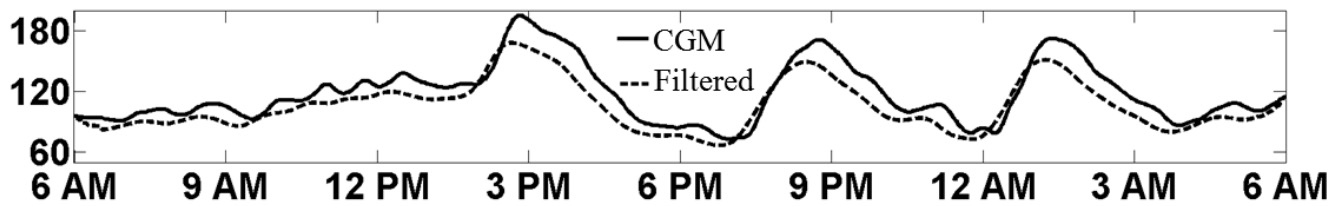
\includegraphics[width=0.6\textwidth]{images/wavelet_example.jpg}
  \caption[]
  {\small Wavelet filter applied on CGM data. Vertical axis represents glocose concentration [mg/dl]. Image courtesy of \textcite{samadi2017}.}
  \label{fig:wavelet_example}
\end{figure}


\subsection{Qualitative Representation}

To identify events in the denoised CGM data feature, extraction is used.
Feature extraction can be acheived by either a qualitative or quantitative method.
The qualitative method offer benefits such as more transparent reasoning and ability to provide explanations for for solutions provided \parencite{Ven2003}.

In qulitative representation by triangular shapes, a CGM data segment can take seven shape variables.
Figure \ref{fig:shapes} shows the different shapes.
Each is a unique combination of the first and second order derivaive on the curve of the current segment.
The derivates can be read from segment adjecent points allowing a CGM data series to be presented as a sequence of shapes describing fluctuations in BG concentration.

\begin{figure}[ht!]
  \centering
  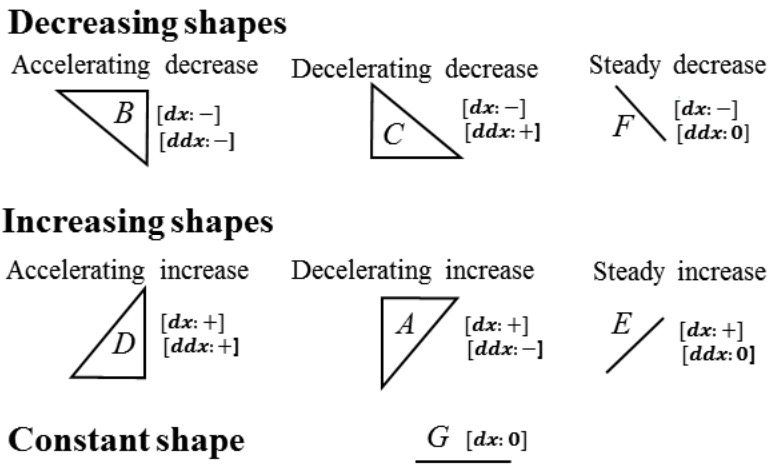
\includegraphics[width=0.6\textwidth]{images/shapes.jpg}
  \caption[]
  {\small Scheme of the qualitative variables A-G. Image courtesy of \textcite{samadi2017}.}
  \label{fig:shapes}
\end{figure}


\subsection{Event Detection}

With the qualitative representation event detection can be performad by analysing the sequence of shapes.
In figure \ref{fig:curve2shape} an event could be triggered by identifying a continously accelerating increase (4 D's in a row from timestep 12).

\begin{figure}[ht!]
  \centering
  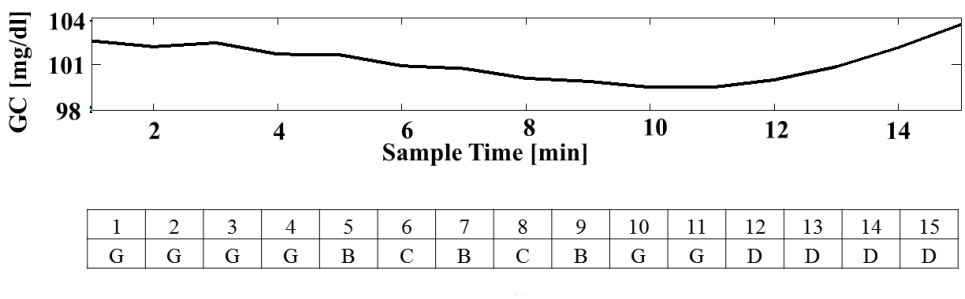
\includegraphics[width=0.8\textwidth]{images/curve2shape.jpg}
  \caption[]
  {\small Shape sequence representation if CGM curve. Image courtesy of \textcite{samadi2017}.}
  \label{fig:curve2shape}
\end{figure}


The detection algorithm could be [INSERT SMART ALG HERE].

\subsection{Intervention Analysis}

Intervention analysis provides a tool to asses how much a given even has changes the series (if at all) \parencite{box2015time}.
The analysis is able to detect 4 patterns:

\begin{enumerate}
  \item Permanent constant change to the mean level.
  \item Brief constant change to the mean level.
  \item Gradual increase or decrase to a new mean level.
  \item Initial change followed by gradual return to previous mean level.
\end{enumerate}

[INSERT INSTERVENTION ANALYSIS MATH HERE]

Because changes in mean BG concentration are subtle and changes naturally takes place over a longer timespan modifications to the original approach need to be made.
I suggest...

\section{Evaluation}

Training/test...

Padova...

Manual labeling...
